\documentclass[border=8mm]{standalone}
\usepackage{tikz}
\usetikzlibrary{calc}

\begin{document}
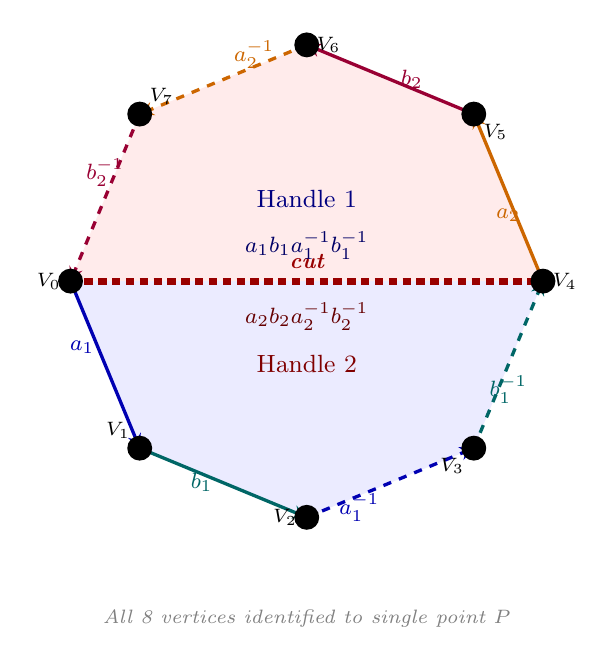
\begin{tikzpicture}[scale=3, line join=round]

% Octagon vertices at 45° intervals, starting at -180°
\foreach \i in {0,...,7} {
  \coordinate (V\i) at ({-180 + \i * 45}:1);
}

% Fill the two halves
% Handle 1 (upper): V0 → V1 → V2 → V3 → V4 → back to V0 via cut
\fill[blue!8] (V0) -- (V1) -- (V2) -- (V3) -- (V4) -- cycle;
% Handle 2 (lower): V4 → V5 → V6 → V7 → V0 → back to V4 via cut
\fill[red!8] (V4) -- (V5) -- (V6) -- (V7) -- (V0) -- cycle;

% Draw octagon sides with identification arrows
% Side 0: a₁ (V0→V1) — thick blue
\draw[->, >=stealth, blue!70!black, line width=1.2pt]
  (V0) -- node[above left, font=\footnotesize\bfseries, blue!70!black] {$a_1$} (V1);

% Side 1: b₁ (V1→V2) — thick teal
\draw[->, >=stealth, teal!80!black, line width=1.2pt]
  (V1) -- node[left, font=\footnotesize\bfseries, teal!80!black] {$b_1$} (V2);

% Side 2: a₁⁻¹ (V2→V3) — thick blue dashed (identified with a₁)
\draw[->, >=stealth, blue!70!black, line width=1.2pt, dashed]
  (V2) -- node[below left, font=\footnotesize\bfseries, blue!70!black] {$a_1^{-1}$} (V3);

% Side 3: b₁⁻¹ (V3→V4) — thick teal dashed
\draw[->, >=stealth, teal!80!black, line width=1.2pt, dashed]
  (V3) -- node[below, font=\footnotesize\bfseries, teal!80!black] {$b_1^{-1}$} (V4);

% Side 4: a₂ (V4→V5) — thick orange
\draw[->, >=stealth, orange!80!black, line width=1.2pt]
  (V4) -- node[below, font=\footnotesize\bfseries, orange!80!black] {$a_2$} (V5);

% Side 5: b₂ (V5→V6) — thick purple
\draw[->, >=stealth, purple!80!black, line width=1.2pt]
  (V5) -- node[right, font=\footnotesize\bfseries, purple!80!black] {$b_2$} (V6);

% Side 6: a₂⁻¹ (V6→V7) — thick orange dashed
\draw[->, >=stealth, orange!80!black, line width=1.2pt, dashed]
  (V6) -- node[above right, font=\footnotesize\bfseries, orange!80!black] {$a_2^{-1}$} (V7);

% Side 7: b₂⁻¹ (V7→V0) — thick purple dashed
\draw[->, >=stealth, purple!80!black, line width=1.2pt, dashed]
  (V7) -- node[above, font=\footnotesize\bfseries, purple!80!black] {$b_2^{-1}$} (V0);

% THE CUT: V0 → V4 diagonal
\draw[red!60!black, line width=2.5pt, densely dashed]
  (V0) -- node[pos=0.5, above, sloped, font=\footnotesize\bfseries\itshape, red!60!black] {cut}
  (V4);

% Vertex dots
\foreach \i in {0,...,7} {
  \fill (V\i) circle (1.5pt);
}

% Vertex labels (all identified to P)
\node[left, font=\scriptsize] at (V0) {$V_0$};
\node[above left, font=\scriptsize] at (V1) {$V_1$};
\node[left, font=\scriptsize] at (V2) {$V_2$};
\node[below left, font=\scriptsize] at (V3) {$V_3$};
\node[right, font=\scriptsize] at (V4) {$V_4$};
\node[below right, font=\scriptsize] at (V5) {$V_5$};
\node[right, font=\scriptsize] at (V6) {$V_6$};
\node[above right, font=\scriptsize] at (V7) {$V_7$};

% Handle labels
\node[font=\small, blue!50!black] at (0, 0.35) {Handle 1};
\node[font=\footnotesize, blue!40!black] at (0, 0.15) {$a_1 b_1 a_1^{-1} b_1^{-1}$};
\node[font=\small, red!50!black] at (0, -0.35) {Handle 2};
\node[font=\footnotesize, red!40!black] at (0, -0.15) {$a_2 b_2 a_2^{-1} b_2^{-1}$};

% Note: all vertices identified
\node[anchor=north, font=\scriptsize\itshape, gray] at (0, -1.35)
  {All 8 vertices identified to single point $P$};

\end{tikzpicture}
\end{document}
